\documentclass[10pt]{article}
\usepackage{amsmath}
\usepackage[colorlinks=true,linkcolor=cyan,citecolor=magenta]{hyperref}
\usepackage{graphicx}
%\usepackage{showframe}

\title{A treatise on phenomenological models of surface second-harmonic
generation from crystalline surfaces}
\author{Bernardo S. Mendoza and Sean M. Anderson}
\date{\today}

\begin{document}
\maketitle
\tableofcontents
\pagebreak

\section{Three layer model for SHG radiation}

In this section we derive the formulas required for the calculation of the SHG
yield, defined by
\begin{align}\label{uno}
R(\omega)=\frac{I(2\omega)}{I^2(\omega)}
,
\end{align}
with the intensity
\begin{align}\label{dos}
I(\omega)=\frac{c}{2\pi}|E(\omega)|^2
,
\end{align}
There are several ways to calculate $R$, one of which is the procedure followed
by Cini \cite{ciniPRB91}. This approach calculates the nonlinear susceptibility
and at the same time the radiated fields. However, we present an alternative
derivation based in the work of Mizrahi and Sipe \cite{mizrahiJOSA88}, since
the derivation of the three-layer-model is straightforward. Within our level of
approximation this is the best model that we can use. In this scheme, we assume
that the SH conversion takes place in a thin layer, just below the surface,
that is characterized by a surface dielectric function
$\epsilon_{\ell}(\omega)$. This layer is below vacuum and sits on top of the
bulk characterized by $\epsilon_{b}(\omega)$ (see Fig. \ref{3layer}). The
nonlinear polarization immersed in the thin layer, will radiate an electric
field directly into vacuum and also into the bulk. This bulk directed field,
will be reflected back into vacuum. Thus, the total field radiated into vacuum
will be the sum of these two contributions (see Fig. \ref{3layer}). We
decompose the field into $s$ and $p$ polarizations, then the electric field
radiated by a polarization sheet,
\begin{align}\label{tres}
\mathcal{P}_i(2\omega)=\chi_{ijk}E_{j}(\omega)E_{k}(\omega)
,
\end{align}
is given by \cite{mizrahiJOSA88},
\begin{equation}\label{r2}
(E_{p\pm},E_s) = 
(\frac{2\pi i\tilde{\omega}^2}{w}
\,\hat{\mathbf{p}}_\pm\cdot\boldsymbol{\mathcal{P}},
\frac{2\pi i\tilde{\omega}^2}{w}
\,\hat{\mathbf{s}}\cdot\boldsymbol{\mathcal{P}}),
\end{equation}
where $\hat{\mathbf{s}}$ and $\hat{\mathbf{p}}_\pm$ are the unitary vectors for
$s$ and $p$ polarization, respectively, and the $\pm$ refers to upward ($+$) or
downward ($-$) direction of propagation. Also, $\tilde\omega=\omega/c$ and
$w_i=\tilde\omega k_i$, with
\begin{equation}\label{r3}
k_i(\omega)=\sqrt{\epsilon_i(\omega) - \sin^2\theta_i},
\end{equation}
where $i=v,\ell,b$, with
\begin{equation}\label{r4}
\hat{\mathbf{p}}_{i\pm} =
\frac{\mp k_i(\omega)\hat{\mathbf{x}} + \sin\theta_i\hat{\mathbf{z}}}
{\sqrt{\epsilon_i(\omega)}}
\end{equation}
\begin{figure}[t]
\centering
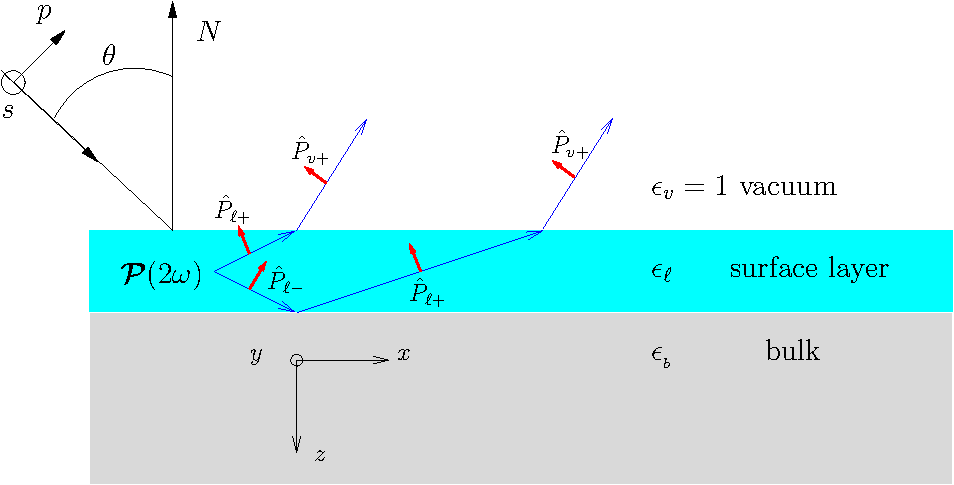
\includegraphics[scale=.5]{figures/3layers}
\caption{Sketch of the three layer model for SHG. Vacuum is on top with
$\epsilon=1$, the layer with nonlinear polarization $\mathbf{P}(2\omega)$
ischaracterized with $\epsilon_{\ell}(\omega)$ and the bulk with
$\epsilon_{b}(\omega)$. In the dipolar approximation the bulk does not radiate
SHG. The thin arrows are along the direction of propagation, and the unit
vectors for $p$-polarization are denoted with thick arrows (capital letters
denote SH components). The unit vector for $s$-polarization points along $-y$
(out of the page).}
\label{3layer}
\end{figure}

In the above equations $z$ is the direction perpendicular to the surface that
points towards the vacuum, $x$ is parallel to the surface, and $\theta$ is the
angle of incidence, where the plane of incidence is chosen as the $xz$ plane
(see Fig. \ref{3layer}), thus $\hat{\mathbf{s}}=-\hat{\mathbf{y}}$. The
function $k_i(\omega)$ is the projection of the wave vector perpendicular to
the surface. As we see from Fig. \ref{3layer}, the SH field is refracted at the
layer-vacuum interface ($\ell v$), and reflected from the layer-bulk ($\ell b$)
interface, thus we can define the transmission, $\mathbf{T}$, and reflection,
$\mathbf{R}$, tensors as,
\begin{equation}\label{r5}
\mathbf{T}_{\ell v}
= \hat{\mathbf{s}}T_s^{\ell v}\hat{\mathbf{s}} 
+ \hat{\mathbf{P}}_{v+}T_{p}^{\ell v} \hat{\mathbf{P}}_{\ell +},
\end{equation}
and
\begin{equation}\label{r6}
\mathbf{R}_{\ell b}
= \hat{\mathbf{s}}R_s^{\ell b}\hat{\mathbf{s}}
+ \hat{\mathbf{P}}_{\ell +}R_{p}^{\ell b} \hat{\mathbf{P}}_{\ell -},
\end{equation}
where variables in capital letters are evaluated at the harmonic frequency
$2\omega$. Notice that since $\hat{\mathbf{s}}$ is independent of $\omega$,
then $\hat{\mathbf{S}}=\hat{\mathbf{s}}$. The Fresnel factors, $T_i$, $R_i$,
for $i=s,p$ polarization, are evaluated at the appropriate interface $\ell v$
or $\ell b$, and will be given below. The extra subscript in $\hat{\mathbf{P}}$
denotes the corresponding dielectric function to be used in its evaluation,
i.e. $\epsilon_v=1$ for vacuum ($v$), $\epsilon_{\ell}$ for the layer ($\ell$),
and $\epsilon_{b}$ for the bulk ($b$). Therefore, the total radiated field at
$2\omega$ is
\begin{align}\label{r7}
\mathbf{E}(2\omega)
&= E_s(2\omega)
\left(
\mathbf{T}^{\ell v} + \mathbf{T}^{\ell v}\cdot\mathbf{R}^{\ell b}
\right)
\cdot\hat{\mathbf{s}}\nonumber\\
&+ E_{p+}(2\omega)\mathbf{T}^{\ell v}\cdot\hat{\mathbf{P}}_{\ell +}
 + E_{p-}(2\omega)\mathbf{T}^{\ell v}
\cdot\mathbf{R}^{\ell b}\cdot\hat{\mathbf{P}}_{\ell-}.
\end{align}
The first term is  the transmitted $s$-polarized field, the second one is the
reflected and then transmitted $s$-polarized field and the third and fourth
terms are the equivalent fields for $p$-polarization. The transmission is from
the layer into vacuum, and the reflection between the layer and the bulk. After
some simple algebra, we obtain
\begin{equation}\label{r8}
\mathbf{E}(2\omega) = \frac{2\pi i\tilde{\Omega}}{K_{\ell}}
\mathbf{H}_{\ell}\cdot\boldsymbol{\mathcal{P}}(2\omega),
\end{equation}
where,
\begin{equation}\label{r9}
\mathbf{H}_{\ell}
= \hat{\mathbf{s}}\,T_s^{\ell v}\left(1+R_s^{\ell b}\right)\hat{\mathbf{s}}
+ \hat{\mathbf{P}}_{v+}T_{p}^{\ell v}
\left(
\hat{\mathbf{P}}_{\ell +} +R_{p}^{\ell b}\hat{\mathbf{P}}_{\ell -}
\right). 
\end{equation}
The magnitude of the radiated field is given by
$E(2\omega)=\hat{\mathbf{e}}^{\mathrm{out}}\cdot\mathbf{E}(2\omega)$, where
$\hat{\mathbf{e}}^{\mathrm{out}}$ is the polarization vector of the radiated
field, for instance $\hat{\mathbf{s}}$ or $\hat{\mathbf{P}}_{v+}$. Then, we
write
\begin{align}\label{m1}
\hat{\mathbf{P}}_{\ell +} + R_{p}^{\ell b}\hat{\mathbf{P}}_{\ell -}
&= \frac{\sin\theta_{\ell}\hat{z} - K_{\ell}\hat{x}}
        {\sqrt{\epsilon_{\ell}(2\omega)}}
 + R_{p}^{\ell b}
   \frac{\sin\theta_{\ell}\hat{z} + K_{\ell}\hat{x}}
        {\sqrt{\epsilon_{\ell}(2\omega)}}
\\\nonumber
&= \frac{1}{\sqrt{\epsilon_{\ell}(2\omega)}}
\left(
\sin\theta_{\ell}(1+R^{\ell b}_{p})\hat{z} - K_{\ell}(1-R^{\ell b}_{p})\hat{x} 
\right)
\\\nonumber 
&= \frac{T^{\ell b}_{p}}{\epsilon_{\ell}(2\omega)\sqrt{\epsilon_{b}(2\omega)}}
\left(
  \epsilon_{b}(2\omega)\sin\theta_{\ell}\hat{z} 
- \epsilon_{\ell}(2\omega)K_{b}\hat{x}
\right)
,
\end{align}
where using
\begin{align}
1 + R^{\ell b}_{s} &= T^{\ell b}_{s}\nonumber\\
1 + R^{\ell b}_{p}
&= \sqrt{\frac{\epsilon_{b}(2\omega)}{\epsilon_{\ell}(2\omega)}}T^{\ell b}_{p} 
\nonumber\\
1 - R^{\ell b}_{p}
&= \sqrt{\frac{\epsilon_{\ell}(2\omega)}{\epsilon_{b}(2\omega)}}
   \frac{K_{b}}{K_{\ell}}T^{\ell b}_{p}\nonumber\\
T^{\ell v}_{p} &= \frac{K_{\ell}}{K_{v}}T^{v\ell}_{p}\nonumber\\
T^{\ell v}_{s} &= \frac{K_{\ell}}{K_{v}}T^{v\ell}_{s}
,
\end{align}
we can write
\begin{equation}\label{r10}
E(2\omega) = \frac{4\pi i \omega}{cK_{v}}
\hat{\mathbf{e}}^{\mathrm{out}}\cdot
\mathbf{H}_{\ell}\cdot
\boldsymbol{\mathcal{P}}(2\omega) 
= \frac{4\pi i\omega}{cK_{v}}
  \mathbf{e}^{\,2\omega}_{\ell}\cdot\boldsymbol{\mathcal{P}}(2\omega). 
\end{equation}
where,
\begin{equation}\label{r12}
\mathbf{e}^{\,2\omega}_{\ell} = \hat{\mathbf{e}}^{\mathrm{out}}\cdot
\left[
\hat{\mathbf{s}}T_{s}^{v\ell}T_{s}^{\ell b}\hat{\mathbf{s}}
+ \hat{\mathbf{P}}_{v+}
\frac{T^{v\ell}_{p}T^{\ell b}_{p}}
     {\epsilon_{\ell}({2\omega})\sqrt{\epsilon_{b}(2\omega)}}
\left(
  \epsilon_{b}(2\omega)\sin\theta_{\ell}\hat{\mathbf{z}}
- \epsilon_{\ell}(2\omega)K_{b}\hat{\mathbf{x}}
\right)
\right]
.  
\end{equation}  
We mention that $n_v\sin\theta_{\mathrm{in}}=n_{\ell}\sin\theta_{\ell}$, from
which $\sin\theta_{\ell}=\sin\theta_{\mathrm{in}}/n_{\ell}$ with
$n_i=\sqrt{\epsilon_i(\omega)}$.

We pause here to reduce above result to the case where the nonlinear
polarization $\mathbf{P}(2\omega)$ radiates from vacuum instead from the layer
$\ell$. For such case we simply take $\epsilon_{\ell}(2\omega)=1$ and $\ell=v$
($T^{\ell v}_{s,p}=1$), to get
\begin{equation}\label{r13}
\mathbf{e}^{\,2\omega}_{v} = \hat{\mathbf{e}}^{\mathrm{out}}
\cdot\left[
\hat{\mathbf{s}}T_s^{v b}\hat{\mathbf{s}} + \hat{\mathbf{P}}_{v+}
\frac{T^{v b}_{p}}{\sqrt{\epsilon_{b}(2\omega)}}
\left(
  \epsilon_{b}(2\omega)\sin\theta_{\mathrm{in}}\hat{\mathbf{z}}
  - K_{b}\hat{\mathbf{x}}
\right) 
\right] 
,
\end{equation}
which agrees with Eq. (3.8) of Ref. \cite{mizrahiJOSA88}.

In the three layer model the nonlinear polarization is located in layer $\ell$,
and then we evaluate the fundamental field required in Eq. \eqref{tres} in this
layer as well, then we write
\begin{equation}\label{m2}
\mathbf{E}_{\ell}(\omega)=E_0\left(
\hat{\mathbf{s}} t^{v\ell}_s(1+r^{\ell b}_s)\hat{\mathbf{s}}
+
\hat{\mathbf{p}}_{\ell-}
 t^{v\ell}_{p}
\hat{\mathbf{p}}_{v-}
+
\hat{\mathbf{p}}_{\ell+}
t^{v\ell}_{p}r^{\ell b}_{p}
\hat{\mathbf{p}}_{v-}
\right)\cdot\hat{\mathbf{e}}^{\mathrm{in}}=E_0\mathbf{e}^\omega_{\ell}
,
\end{equation} 
and following the steps that lead to Eq. \eqref{r12}, we find that
\begin{equation}\label{m12}
\mathbf{e}^{\omega}_{\ell}
= \left[
\hat{\mathbf{s}}t_{s}^{v\ell}t_{s}^{\ell b}\hat{\mathbf{s}} 
+ \frac{t^{v\ell}_{p}t^{\ell b}_{p}}
       {\epsilon_{\ell}(\omega)\sqrt{\epsilon_{b}(\omega)}}
\left(
  \epsilon_{b}(\omega)\sin\theta_{\ell}\hat{\mathbf{z}}
+ \epsilon_{\ell}(\omega)k_{b}\hat{\mathbf{x}}
\right)
\hat{\mathbf{p}}_{v-}
\right]
\cdot\hat{\mathbf{e}}^{\mathrm{in}}.  
\end{equation}  
If we would like to evaluate the fields in the bulk, instead of the
layer $\ell$, we simply take 
$\epsilon_{\ell}(\omega)=\epsilon_{b}(\omega)\,(t^{\ell b}_{s,p}=1$), to obtain 
\begin{equation}\label{m13}
\mathbf{e}^{\omega}_{b}
= \left[
\hat{\mathbf{s}}t_{s}^{vb}\hat{\mathbf{s}}
+ \frac{t^{vb}_{p}}{\sqrt{\epsilon_{b}(\omega)}}
\left(
\sin\theta_{\mathrm{in}}\hat{\mathbf{z}} + k_{b}\hat{\mathbf{x}}
\right) 
\hat{\mathbf{p}}_{v-}
\right]
\cdot\hat{\mathbf{e}}^{\mathrm{in}},  
\end{equation} 
that is in agreement with Eq. (3.5) of Ref. \cite{mizrahiJOSA88}.

With $\mathbf{e}^{\omega}$ we can write Eq. \eqref{tres} as
\begin{equation}\label{m4}
\boldsymbol{\mathcal{P}}(2\omega) = E^{2}_{0}\boldsymbol{\chi}:
\mathbf{e}^{\omega}_{\ell}\mathbf{e}^{\omega}_{\ell}
,
\end{equation}
and then from Eq. \eqref{r10} we obtain that
\begin{align}\label{r01}
|E(2\omega)|^2 
&= |E_{0}|^4\frac{16\pi^{2}\omega^{2}}{c^{2}K^{2}_{v}}
\left\vert
\mathbf{e}^{\,2\omega}_{\ell}\cdot\boldsymbol{\chi}:
\mathbf{e}^{\omega}_{\ell}\mathbf{e}^{\omega}_{\ell}
\right\vert^{2}
\nonumber\\
\frac{c}{2\pi}|E(2\omega)|^{2} 
&= \frac{32\pi^{3}\omega^{2}}{c^{3}\cos^{2}\theta_{\mathrm{in}}}
\left\vert
\mathbf{e}^{\,2\omega}_{\ell}\cdot\boldsymbol{\chi}:
\mathbf{e}^{\omega}_{\ell}\mathbf{e}^{\omega}_{\ell}
\right\vert^{2} 
\left(\frac{c}{2\pi}|E_{0}|^{2}\right)^{2},
\nonumber\\
I(2\omega) 
&= \frac{32\pi^{3}\omega^{2}}{c^{3}\cos^{2}\theta_{\mathrm{in}}}
\left\vert
\mathbf{e}^{\,2\omega}_{\ell}\cdot\boldsymbol{\chi}:
\mathbf{e}^\omega_{\ell}\mathbf{e}^\omega_{\ell}
\right\vert^{2}I^{2}(\omega),
\nonumber\\
R(2\omega) 
&= \frac{32\pi^{3}\omega^{2}}{c^{3}\cos^{2}\theta_{\mathrm{in}}}
\left\vert
\mathbf{e}^{\,2\omega}_{\ell}\cdot\boldsymbol{\chi}:
\mathbf{e}^{\omega}_{\ell}\mathbf{e}^{\omega}_{\ell}\right\vert^{2} 
,
\end{align}
as the SHG yield. At this point we mention that to recover the results of Ref.
\cite{mizrahiJOSA88} which are equivalent of those of Ref. \cite{sipePRB87}, we
take $\mathbf{e}^{2\omega}_{\ell}\to \mathbf{e}^{2\omega}_v$,
$\mathbf{e}^{\omega}_{\ell}\to \mathbf{e}^{\omega}_{b}$ and then
\begin{equation}\label{m69}
R(2\omega) =
\frac{32\pi^{3} \omega^{2}}{c^{3}\cos^{2}\theta_{\mathrm{in}}}
\left\vert
\mathbf{e}^{\,2\omega}_{v}\cdot\boldsymbol{\chi}:
\mathbf{e}^{\omega}_{b}\mathbf{e}^{\omega}_{b}
\right\vert^{2} 
,
\end{equation}
will give the SHG yield of a nonlinear polarization sheet radiating from vacuum
on top of the surface and where the fundamental field is evaluated below the
surface that is characterized by $\epsilon_{b}(\omega)$.

To complete the required formulas, we write down the Fresnel factors,
\begin{equation}\label{e.f1}
\begin{split}
t_s^{ij}(\omega) &=
\frac{2k_{i}(\omega)}{k_{i}(\omega)+k_{j}(\omega)},
\quad\quad  
t_{p}^{ij}(\omega) =
\frac{2k_{i}(\omega)\sqrt{\epsilon_{i}(\omega)\epsilon_j(\omega)}}
     {k_{i}(\omega)\epsilon_{j}(\omega)+k_{j}(\omega)\epsilon_{i}(\omega)},\\
r_s^{ij}(\omega) &=
\frac{k_{i}(\omega) - k_{j}(\omega)}
     {k_{i}(\omega) + k_{j}(\omega)},
\quad\quad 
r_{p}^{ij}(\omega) =
\frac{k_{i}(\omega)\epsilon_{j}(\omega) - k_{j}\epsilon_{i}(\omega)}
     {k_{i}(\omega)\epsilon_{j}(\omega) + k_{j}(\omega)\epsilon_{i}(\omega)}.
\end{split}
\end{equation}


\section{\texorpdfstring{$\mathcal{R}$}{R} for different polarization cases}

We obtain explicit relations for a $C_{3v}$ symmetry characteristic of a (111)
surface, for which the only components of $\chi_{ijk}$ different from zero are
$\chi_{zzz}$, $\chi_{zxx}=\chi_{zyy}$, $\chi_{xxz}=\chi_{yyz}$ and
$\chi_{xxx}=-\chi_{xyy}=-\chi_{yyx}$ with $\chi_{ijk}=\chi_{ikj}$, where we
have chosen the $x$ and $y$ axes along the [112] and [110] directions,
respectively.

However, we have to remember that the plane of incidence so far was chosen to
be the $xz$ plane; the most general plane of incidence should be one that makes
an angle $\phi$ with respect to the $x$ axis, and so $\hat{\mathbf{x}}$ should
to be replaced by a unit vector $\hat{\mathbf{\kappa}}$ such that
\begin{equation}\label{mc1}
\hat{\boldsymbol{\kappa}}
= \cos\phi\hat{\mathbf{x}} + \sin\phi\hat{\mathbf{y}},
\end{equation}
and then
\begin{equation}\label{mc2}
\hat{\mathbf{s}} = -\sin\phi\hat{\mathbf{x}} + \cos\phi\hat{\mathbf{y}},
\end{equation}

\subsection{\texorpdfstring{$\mathcal{R}_{pP}$}{RpP}}

To obtain $R_{pP}(2\omega)$ we use
$\mathbf{e}^{\mathrm{in}}=\hat{\mathbf{p}}_{v-}$ in Eq. \eqref{m12}, and
$\mathbf{e}^{\mathrm{out}}=\hat{\mathbf{P}}_{v+}$ in Eq. \eqref{r12}, to obtain
that for a $C_{3v}$ symmetry characteristic of a (111) surface,
\begin{equation*}\label{m80}
\mathbf{e}^{\,2\omega}_{\ell}\cdot\boldsymbol{\chi}:
\mathbf{e}^\omega_{\ell}\mathbf{e}^\omega_{\ell}
\equiv\Gamma^{\ell}_{pP}\,r^{\ell}_{pP}
,
\end{equation*}
where
\begin{equation*}\label{m81}
\begin{split}
r^{\ell}_{pP} &=
\epsilon_{b}(2\omega)\sin\theta_{\ell}
\Big(
  \epsilon^2_{b}(\omega)\sin^2\theta_{\ell}\chi_{zzz}
+ \epsilon^2_{\ell}(\omega) k^2_{b}(\omega)\chi_{zxx}
\Big)\nonumber\\
&- \epsilon_{\ell}(2\omega)\epsilon_{\ell}(\omega)k_{b}(\omega)k_{b}(2\omega)
\Big(
  2\epsilon_{b}(\omega)\sin\theta_{\ell}\chi_{xxz}
+ \epsilon_{\ell}(\omega)k_{b}(\omega)\chi_{xxx}\cos(3\phi) 
\Big),
\end{split} 
\end{equation*}
and  
\begin{equation*}\label{m79}
\Gamma^{\ell}_{pP}=
\frac{T_{p}^{\ell v}T^{\ell b}_{p}}
     {\epsilon_{\ell}(2\omega)\sqrt{\epsilon_{b}(2\omega)}}
\left(
\frac{t_{p}^{v\ell}t^{\ell b}_{p}}
     {\epsilon_{\ell}(\omega)\sqrt{\epsilon_{b}(\omega)}}
\right)^{2} 
.  
\end{equation*} 
In order to reduce above result to that of Ref. \cite{mizrahiJOSA88} and
\cite{sipePRB87},  we take the 2-$\omega$ radiations factors for vacuum by
taking $\ell=v$, thus $\epsilon_{\ell}(2\omega)=1$, $T^{\ell v}_{p}=1$,
$T^{\ell b}_{p}=T^{vb}_{p}$, and the fundamental field inside medium $b$ by
taking $\ell=b$, thus $\epsilon_{\ell}(\omega)=\epsilon_{b}(\omega)$,
$t^{v\ell}_{p}=t^{vb}_{p}$, $t^{\ell b}_{p}=1$ and
$\theta_{\ell}=\theta_{\mathrm{in}}$. With these choices,
\begin{equation*}\label{m82}
\begin{split}
r^{b}_{pP}
&= \epsilon_{b}(2\omega)\sin\theta_{\mathrm{in}}
\Big(
\sin^2\theta_{\mathrm{in}}\chi_{zzz} + k^{2}_{b}(\omega)\chi_{zxx}
\Big)\nonumber\\
&- k_{b}(\omega)k_{b}(2\omega)
\Big(
2\sin\theta_{\mathrm{in}}\chi_{xxz} + k_{b}(\omega)\chi_{xxx}\cos(3\phi) 
\Big) 
,
\end{split}
\end{equation*}
and 
\begin{equation*}\label{m78}
\Gamma^b_{pP}
= \frac{T^{v b}_{p}(t^{vb}_{p})^2}
       {\epsilon_{b}(\omega)\sqrt{\epsilon_{b}(2\omega)}}
.
\end{equation*}


\subsection{\texorpdfstring{$\mathcal{R}_{pS}$}{RpS}}

To obtain $R_{pS}(2\omega)$ we use
$\mathbf{e}^{\mathrm{in}}=\hat{\mathbf{p}}_{v-}$ in Eq. \eqref{m12}, and
$\mathbf{e}^{\mathrm{out}}=\hat{\mathbf{S}}$ in Eq. \eqref{r12}. We also use
the unit vectors defined in Eqs. \eqref{mc1} and
\eqref{mc2}. Substituting, we get
\begin{equation*}
\hat{\mathbf{e}}^{2\omega}_{\ell} 
= T^{v\ell}_{s}T^{\ell b}_{s}
\left[-\sin\phi\hat{\mathbf{x}} + \cos\phi\hat{\mathbf{y}}\right],
\end{equation*}
for $2\omega$, and for the fundamental fields,
\begin{align*}
\hat{\mathbf{e}}^{\omega}_{\ell}\hat{\mathbf{e}}^{\omega}_{\ell}
= \left(
\frac{t^{v\ell}_{p}t^{\ell b}_{p}}
       {\epsilon_{\ell}(\omega)\sqrt{\epsilon_{b}(\omega)}}
\right)^{2}
&\left(
  \epsilon_{b}(\omega)\sin\theta_{\ell}\hat{\mathbf{z}}
+ \epsilon_{\ell}(\omega)k_{b}\cos\phi\hat{\mathbf{x}}
+ \epsilon_{\ell}(\omega)k_{b}\sin\phi\hat{\mathbf{y}}
\right)^{2}.\\
= \left(
\frac{t^{v\ell}_{p}t^{\ell b}_{p}}
       {\epsilon_{\ell}(\omega)\sqrt{\epsilon_{b}(\omega)}}
\right)^{2}
&\big(
  \epsilon_{b}^{2}(\omega)\sin^{2}\theta_{\ell}\hat{\mathbf{z}}\hat{\mathbf{z}}
+ 2\epsilon_{b}(\omega)\epsilon_{\ell}(\omega)k_{b}\sin\theta_{\ell}
   \cos\phi\hat{\mathbf{z}}\hat{\mathbf{x}}\\
+ &\epsilon^{2}_{\ell}(\omega)k^{2}_{b}\cos^{2}\phi
   \hat{\mathbf{x}}\hat{\mathbf{x}}
+ 2\epsilon^{2}_{\ell}(\omega)k^{2}_{b}\cos\phi\sin\phi
   \hat{\mathbf{x}}\hat{\mathbf{y}}\\
+ &\epsilon^{2}_{\ell}(\omega)k^{2}_{b}\sin^{2}\phi
   \hat{\mathbf{y}}\hat{\mathbf{y}}
+ 2\epsilon_{b}(\omega)\epsilon_{\ell}(\omega)k_{b}\sin\theta_{\ell}\sin\phi
   \hat{\mathbf{y}}\hat{\mathbf{z}}
\big).
\end{align*}
Therefore,
\begin{equation*}
\begin{split}
\hat{\mathbf{e}}^{2\omega}_{\ell}
\cdot\boldsymbol{\chi}:
\hat{\mathbf{e}}^{\omega}_{\ell}\hat{\mathbf{e}}^{\omega}_{\ell} =
\qquad\qquad\qquad&\\\\
T^{v\ell}_{s}T^{\ell b}_{s}\left(\frac{t^{v\ell}_{p}t^{\ell b}_{p}}
      {\epsilon_{\ell}(\omega)\sqrt{\epsilon_{b}(\omega)}}\right)^{2}
\big[
- &\epsilon_{b}^{2}(\omega)\sin^{2}\theta_{\ell}\sin\phi\chi_{xzz}\\
-&2\epsilon_{b}(\omega)\epsilon_{\ell}(\omega)k_{b}\sin\theta_{\ell}
   \cos\phi\sin\phi\chi_{xxz}\\
- &\epsilon^{2}_{\ell}(\omega)k^{2}_{b}\cos^{2}\phi\sin\phi\chi_{xxx}\\
-&2\epsilon^{2}_{\ell}(\omega)k^{2}_{b}\cos\phi\sin^{2}\phi\chi_{xxy}\\
- &\epsilon^{2}_{\ell}(\omega)k^{2}_{b}\sin^{3}\phi\chi_{xyy}\\
-&2\epsilon_{b}(\omega)\epsilon_{\ell}(\omega)k_{b}\sin\theta_{\ell}
   \sin^{2}\phi\chi_{xyz}\\
+ &\epsilon_{b}^{2}(\omega)\sin^{2}\theta_{\ell}\cos\phi\chi_{yzz}\\
+&2\epsilon_{b}(\omega)\epsilon_{\ell}(\omega)k_{b}\sin\theta_{\ell}
   \cos^{2}\phi\chi_{yxz}\\
+ &\epsilon^{2}_{\ell}(\omega)k^{2}_{b}\cos^{3}\phi\chi_{yxx}\\
+&2\epsilon^{2}_{\ell}(\omega)k^{2}_{b}\cos^{2}\phi\sin\phi\chi_{yxy}\\
+ &\epsilon^{2}_{\ell}(\omega)k^{2}_{b}\cos\phi\sin^{2}\phi\chi_{yyy}\\
+&2\epsilon_{b}(\omega)\epsilon_{\ell}(\omega)k_{b}\sin\theta_{\ell}
   \cos\phi\sin\phi\chi_{yyz}
\big],
\end{split}
\end{equation*}
and taking into account that $\chi_{xzz} = \chi_{xxy} = \chi_{xyz} = \chi_{yzz}
= \chi_{yxz} = \chi_{yxx} = \chi_{yyy} = 0$, we have
\begin{equation*}
\begin{split}
= \Gamma^{\ell}_{pS}
\big[
+ &\epsilon^{2}_{\ell}(\omega)k^{2}_{b}\sin^{3}\phi\chi_{xxx}\\
-&2\epsilon^{2}_{\ell}(\omega)k^{2}_{b}\cos^{2}\phi\sin\phi\chi_{xxx}\\
- &\epsilon^{2}_{\ell}(\omega)k^{2}_{b}\cos^{2}\phi\sin\phi\chi_{xxx}\\
+&2\epsilon_{b}(\omega)\epsilon_{\ell}(\omega)k_{b}\sin\theta_{\ell}
   \cos\phi\sin\phi\chi_{xxz}\\
-&2\epsilon_{b}(\omega)\epsilon_{\ell}(\omega)k_{b}\sin\theta_{\ell}
   \cos\phi\sin\phi\chi_{xxz}
\big]\\\\
= \Gamma^{\ell}_{pS}
\big[
&\epsilon^{2}_{\ell}(\omega)k^{2}_{b}
(\sin^{3}\phi - 3\cos^{2}\phi\sin\phi)\chi_{xxx}
\big]\\\\
= \Gamma^{\ell}_{pS}
\big[
&-\epsilon^{2}_{\ell}(\omega)k^{2}_{b}
\sin3\phi\chi_{xxx}
\big].
\end{split}
\end{equation*}
We summarize as follows,
\begin{equation*}
\mathbf{e}^{\,2\omega}_{\ell}\cdot
\boldsymbol{\chi}:\mathbf{e}^\omega_{\ell}\mathbf{e}^\omega_{\ell}
\equiv\Gamma^{\ell}_{sP}\, r^{\ell}_{sP},
\end{equation*}
where
\begin{equation*}
r^{\ell}_{pS}
= -\epsilon^{2}_{\ell}(\omega)k^{2}_{b}\sin3\phi\chi_{xxx},
\end{equation*} 
and  
\begin{equation*}
\Gamma^{\ell}_{pS} =
T^{v\ell}_{s}T^{\ell b}_{s}\left(\frac{t^{v\ell}_{p}t^{\ell b}_{p}}
      {\epsilon_{\ell}(\omega)\sqrt{\epsilon_{b}(\omega)}}\right)^{2}
\end{equation*} 
In order to reduce above result to that of Ref. \cite{mizrahiJOSA88} and
\cite{sipePRB87},  we take the 2-$\omega$ radiations factors for vacuum by
taking $\ell=v$, thus $\epsilon_{\ell}(2\omega)=1$, $T^{v\ell}_{s}=1$,
$T^{\ell b}_{s}=T^{vb}_{s}$, and the fundamental field inside medium $b$ by
taking $\ell=b$, thus $\epsilon_{\ell}(\omega)=\epsilon_{b}(\omega)$,
$t^{v\ell}_{p}=t^{vb}_{p}$, $t^{\ell b}_{p}=1$ and
$\theta_{\ell}=\theta_{\mathrm{in}}$. With these choices,
\begin{equation*}
r^{b}_{pS} = -k^{2}_{b}\sin3\phi\chi_{xxx},
\end{equation*} 
and 
\begin{equation*}
\Gamma^{b}_{pS} =
T^{vb}_{s}\left(\frac{t^{vb}_{p}}{\epsilon_{b}(\omega)\sqrt{\epsilon_{b}(\omega)}}\right)^{2}.  
\end{equation*} 


\subsection{\texorpdfstring{$\mathcal{R}_{sP}$}{RsP}}

To obtain $R_{sP}(2\omega)$ we use $\mathbf{e}^{\mathrm{in}}=\hat{\mathbf{s}}$
in Eq. \eqref{m12}, and $\mathbf{e}^{\mathrm{out}}=\hat{\mathbf{P}}_{v+}$ in
Eq. \eqref{r12}. We also use the unit vectors defined in Eqs. \eqref{mc1} and
\eqref{mc2}. Substituting, we get
\begin{equation*}
\hat{\mathbf{e}}^{2\omega}_{\ell} 
= \frac{T^{v\ell}_{p}T^{\ell b}_{p}}
       {\epsilon_{\ell}(2\omega)\sqrt{\epsilon_{b}(2\omega)}}
\left[
  \epsilon_{b}(2\omega)\sin\theta_{\ell}\hat{\mathbf{z}} 
- \epsilon_{\ell}(2\omega)K_{b}\cos\phi\hat{\mathbf{x}} 
- \epsilon_{\ell}(2\omega)K_{b}\sin\phi\hat{\mathbf{y}}
\right],
\end{equation*}
for $2\omega$, and for the fundamental fields,
\begin{equation*}
\hat{\mathbf{e}}^{\omega}_{\ell}\hat{\mathbf{e}}^{\omega}_{\ell}
= \left(t^{v\ell}_{s}t^{\ell b}_{s}\right)^{2}
\left(
  \sin^{2}\phi\hat{\mathbf{x}}\hat{\mathbf{x}}
+ \cos^{2}\phi\hat{\mathbf{y}}\hat{\mathbf{y}} 
- 2\sin\phi\cos\phi\hat{\mathbf{x}}\hat{\mathbf{y}}
\right).
\end{equation*}
Therefore,
\begin{equation*}
\begin{split}
\hat{\mathbf{e}}^{2\omega}_{\ell}
\cdot\boldsymbol{\chi}:&
\hat{\mathbf{e}}^{\omega}_{\ell}\hat{\mathbf{e}}^{\omega}_{\ell} =\\
&\frac{T^{v\ell}_{p}T^{\ell b}_{p}\left(t^{v\ell}_{s}t^{\ell b}_{s}\right)^{2}}
      {\epsilon_{\ell}(2\omega)\sqrt{\epsilon_{b}(2\omega)}}
\big[
   \epsilon_{b}(2\omega)\sin\theta_{\ell}\sin^{2}\phi\chi_{zxx} 
 + \epsilon_{b}(2\omega)\sin\theta_{\ell}\cos^{2}\phi\chi_{zyy}\\
&- 2\epsilon_{b}(2\omega)\sin\theta_{\ell}\sin\phi\cos\phi\chi_{zxy}
 - \epsilon_{\ell}(2\omega)K_{b}\cos\phi\sin^{2}\phi\chi_{xxx}\\
&- \epsilon_{\ell}(2\omega)K_{b}\cos\phi\cos^{2}\phi\chi_{xyy}
 + 2\epsilon_{\ell}(2\omega)K_{b}\cos\phi\sin\phi\cos\phi\chi_{xxy}\\
&- \epsilon_{\ell}(2\omega)K_{b}\sin\phi\sin^{2}\phi\chi_{yxx}
 - \epsilon_{\ell}(2\omega)K_{b}\sin\phi\cos^{2}\phi\chi_{yyy}\\
&+ 2\epsilon_{\ell}(2\omega)K_{b}\sin\phi\sin\phi\cos\phi\chi_{yxy}
\big],
\end{split}
\end{equation*}
and taking into account that $\chi_{zxy} = \chi_{xxy} = \chi_{yxx} = \chi_{yyy}
= 0$, we have
\begin{equation*}
\begin{split}
= \Gamma^{\ell}_{sP}
&\big[
   \epsilon_{b}(2\omega)\sin\theta_{\ell}\sin^{2}\phi\chi_{zxx}
 + \epsilon_{b}(2\omega)\sin\theta_{\ell}\cos^{2}\phi\chi_{zxx}\\
&- \epsilon_{\ell}(2\omega)K_{b}\cos\phi\sin^{2}\phi\chi_{xxx}
 + \epsilon_{\ell}(2\omega)K_{b}\cos^{3}\phi\chi_{xxx}\\
&- 2\epsilon_{\ell}(2\omega)K_{b}\sin^{2}\phi\cos\phi\chi_{xxx}
\big]\\\\
= \Gamma^{\ell}_{sP}
&\big[
\epsilon_{b}(2\omega)\sin\theta_{\ell}
(\sin^{2}\phi + \cos^{2}\phi)\chi_{zxx}\\
&- \epsilon_{\ell}(2\omega)K_{b}
(\cos\phi\sin^{2}\phi - \cos^{3}\phi + 2\sin^{2}\phi\cos\phi)\chi_{xxx}
\big]\\\\
= \Gamma^{\ell}_{sP}
&\big[
  \epsilon_{b}(2\omega)\sin\theta_{\ell}\chi_{zxx} 
+ \epsilon_{\ell}(2\omega)K_{b}(\cos^{3}\phi - 3\sin^{2}\phi\cos\phi)\chi_{xxx}
\big]\\\\
= \Gamma^{\ell}_{sP}
&\big[
  \epsilon_{b}(2\omega)\sin\theta_{\ell}\chi_{zxx}
+ \epsilon_{\ell}(2\omega)K_{b}\cos3\phi\chi_{xxx}
\big].
\end{split}
\end{equation*}
We summarize as follows,
\begin{equation*}
\mathbf{e}^{\,2\omega}_{\ell}\cdot
\boldsymbol{\chi}:\mathbf{e}^\omega_{\ell}\mathbf{e}^\omega_{\ell}
\equiv\Gamma^{\ell}_{sP}\, r^{\ell}_{sP},
\end{equation*}
where
\begin{equation*}
r^{\ell}_{sP}
= \epsilon_{b}(2\omega)\sin\theta_{\ell}\chi_{zxx}
+ \epsilon_{\ell}(2\omega)K_{b}\chi_{xxx}\cos3\phi,
\end{equation*} 
and  
\begin{equation*}
\Gamma^{\ell}_{sP}=
\frac{T_{p}^{\ell v}T^{\ell b}_{p}\left(t_s^{v\ell}t^{\ell b}_s\right)^2}
     {\epsilon_{\ell}(2\omega)\sqrt{\epsilon_{b}(2\omega)}}.  
\end{equation*} 
In order to reduce above result to that of Ref. \cite{mizrahiJOSA88} and
\cite{sipePRB87},  we take the 2-$\omega$ radiations factors for vacuum by
taking $\ell=v$, thus $\epsilon_{\ell}(2\omega)=1$, $T^{v\ell}_{p}=1$,
$T^{\ell b}_{p}=T^{vb}_{p}$, and the fundamental field inside medium $b$ by
taking $\ell=b$, thus $\epsilon_{\ell}(\omega)=\epsilon_{b}(\omega)$,
$t^{v\ell}_s=t^{vb}_s$, $t^{\ell b}_s=1$ and
$\theta_{\ell}=\theta_{\mathrm{in}}$. With these choices,
\begin{equation*}
r^{b}_{sP} = \epsilon_{b}(2\omega)\sin\theta_{\mathrm{in}}\chi_{zxx}
+ K_{b}\chi_{xxx}\cos3\phi,
\end{equation*} 
and 
\begin{equation*}
\Gamma^{b}_{sP} =
\frac{T^{v b}_{p}(t_s^{vb})^{2}}{\sqrt{\epsilon_{b}(2\omega)}}.  
\end{equation*} 


\section{Trials and tribulations}

\subsection{Taking the \texorpdfstring{$2\omega$}{2w} fields in the bulk}

To consider the $2\omega$ fields in the bulk, we start with Eq. \eqref{r9} but
substitute $\ell\rightarrow b$, thus
\begin{equation*}
\mathbf{H}_{b}
= \hat{\mathbf{s}}\,T_s^{b v}\left(1+R_{s}^{b b}\right)\hat{\mathbf{s}}
+ \hat{\mathbf{P}}_{v+}T_{p}^{b v}
\left(
\hat{\mathbf{P}}_{b+} + R_{p}^{b b}\hat{\mathbf{P}}_{b-}
\right).
\end{equation*}
$R_{p}^{b b}$ and $R_{s}^{b b}$ are zero, so we are left with
\begin{equation*}
\begin{split}
\mathbf{H}_{b}
&= \hat{\mathbf{s}}\,T_s^{b v}\hat{\mathbf{s}}
 + \hat{\mathbf{P}}_{v+}T_{p}^{b v}\hat{\mathbf{P}}_{b+}\\
&= \frac{K_{b}}{K_{v}}\left(\hat{\mathbf{s}}\,T_s^{vb}\hat{\mathbf{s}}
 + \hat{\mathbf{P}}_{v+}T_{p}^{vb}\hat{\mathbf{P}}_{b+}\right)\\
&= \frac{K_{b}}{K_{v}}
   \left[
   \hat{\mathbf{s}}\,T_s^{vb}\hat{\mathbf{s}}
 + \hat{\mathbf{P}}_{v+}
   \frac{T_{p}^{vb}}{\sqrt{\epsilon_{b}(2\omega)}}
   (\sin\theta_{\mathrm{in}}\hat{\mathbf{z}}
 - K_{b}\cos\phi\hat{\mathbf{x}} 
 - K_{b}\sin\phi\hat{\mathbf{y}})
   \right],
\end{split}
\end{equation*}
and we define
\begin{equation*}
\mathbf{e}^{\,2\omega}_{b}
= \frac{K_{b}}{K_{v}}\,\hat{\mathbf{e}}^{\mathrm{out}}\cdot
\left[
   \hat{\mathbf{s}}\,T_s^{vb}\hat{\mathbf{s}}
 + \hat{\mathbf{P}}_{v+}
   \frac{T_{p}^{vb}}{\sqrt{\epsilon_{b}(2\omega)}}
   (\sin\theta_{\mathrm{in}}\hat{\mathbf{z}}
 - K_{b}\cos\phi\hat{\mathbf{x}} 
 - K_{b}\sin\phi\hat{\mathbf{y}})
   \right].
\end{equation*}
For $\mathcal{R}_{pP}$, we require
$\hat{\mathbf{e}}^{\mathrm{out}}=\hat{\mathbf{P}}_{v+}$, so we have that
\begin{equation*}
\mathbf{e}^{\,2\omega}_{b}
= \frac{K_{b}}{K_{v}}
  \frac{T_{p}^{vb}}{\sqrt{\epsilon_{b}(2\omega)}}
  (\sin\theta_{\mathrm{in}}\hat{\mathbf{z}}
- K_{b}\cos\phi\hat{\mathbf{x}} 
- K_{b}\sin\phi\hat{\mathbf{y}}).
\end{equation*}

The $1\omega$ fields will still be evaluated inside the bulk, so we have Eq.
\eqref{m13}
\begin{equation*}
\mathbf{e}^{\omega}_{b}
= \left[
\hat{\mathbf{s}}t_{s}^{vb}\hat{\mathbf{s}}
+ \frac{t^{vb}_{p}}{\sqrt{\epsilon_{b}(\omega)}}
\left(
  \sin\theta_{\mathrm{in}}\hat{\mathbf{z}}
+ k_{b}\cos\phi\hat{\mathbf{x}}
+ k_{b}\sin\phi\hat{\mathbf{y}}
\right) 
\hat{\mathbf{p}}_{v-}
\right]
\cdot\hat{\mathbf{e}}^{\mathrm{in}},  
\end{equation*}
and for our particular case of
$\hat{\mathbf{e}}^{\mathrm{in}}=\hat{\mathbf{p}}_{v-}$,
\begin{equation*}
\mathbf{e}^{\omega}_{b}
= \frac{t^{vb}_{p}}{\sqrt{\epsilon_{b}(\omega)}}
\left(
  \sin\theta_{\mathrm{in}}\hat{\mathbf{z}}
+ k_{b}\cos\phi\hat{\mathbf{x}}
+ k_{b}\sin\phi\hat{\mathbf{y}}
\right),
\end{equation*}
and
\begin{equation*}
\begin{split}
\mathbf{e}^{\omega}_{b}\mathbf{e}^{\omega}_{b}
&= \frac{\left(t^{vb}_{p}\right)^{2}}{\epsilon_{b}(\omega)}
\left(
  \sin\theta_{\mathrm{in}}\hat{\mathbf{z}}
+ k_{b}\cos\phi\hat{\mathbf{x}}
+ k_{b}\sin\phi\hat{\mathbf{y}}
\right)^{2}\\
&= \frac{\left(t^{vb}_{p}\right)^{2}}{\epsilon_{b}(\omega)}
\big(
  \sin^{2}\theta_{\mathrm{in}}\hat{\mathbf{z}}\hat{\mathbf{z}}
+ k^{2}_{b}\cos^{2}\phi\hat{\mathbf{x}}\hat{\mathbf{x}}
+ k^{2}_{b}\sin^{2}\phi\hat{\mathbf{y}}\hat{\mathbf{y}}\\
&\qquad\qquad
+ 2k_{b}\sin\theta_{\mathrm{in}}\cos\phi\hat{\mathbf{z}}\hat{\mathbf{x}}
+ 2k_{b}\sin\theta_{\mathrm{in}}\sin\phi\hat{\mathbf{z}}\hat{\mathbf{y}}
+ 2k^{2}_{b}\sin\phi\cos\phi\hat{\mathbf{x}}\hat{\mathbf{y}}
\big)
\end{split}
\end{equation*}

So lastly, we have that
\begin{equation*}
\begin{split}
\mathbf{e}^{\,2\omega}_{b}\cdot
\boldsymbol{\chi}:\mathbf{e}^{\omega}_{b}\mathbf{e}^{\omega}_{b} =
\frac{K_{b}}{K_{v}}
\frac{T_{p}^{vb}\left(t^{vb}_{p}\right)^{2}}
     {\epsilon_{b}(\omega)\sqrt{\epsilon_{b}(2\omega)}}
&\big(
   \sin^{3}\theta_{\mathrm{in}}\chi_{zzz}\\
&+ k^{2}_{b}\sin\theta_{\mathrm{in}}\cos^{2}\phi\chi_{zxx}\\
&+ k^{2}_{b}\sin\theta_{\mathrm{in}}\sin^{2}\phi\chi_{zyy}\\
&+ 2k_{b}\sin^{2}\theta_{\mathrm{in}}\cos\phi\chi_{zzx}\\
&+ 2k_{b}\sin^{2}\theta_{\mathrm{in}}\sin\phi\chi_{zzy}\\
&+ 2k^{2}_{b}\sin\theta_{\mathrm{in}}\sin\phi\cos\phi\chi_{zxy}\\
&- K_{b}\sin^{2}\theta_{\mathrm{in}}\cos\phi\chi_{xzz}\\
&- k^{2}_{b}K_{b}\cos^{3}\phi\chi_{xxx}\\
&- k^{2}_{b}K_{b}\sin^{2}\phi\cos\phi\chi_{xyy}\\
&- 2k_{b}K_{b}\sin\theta_{\mathrm{in}}\cos^{2}\phi\chi_{xzx}\\
&- 2k_{b}K_{b}\sin\theta_{\mathrm{in}}\sin\phi\cos\phi\chi_{xzy}\\
&- 2k^{2}_{b}K_{b}\sin\phi\cos^{2}\phi\chi_{xxy}\\
&- K_{b}\sin^{2}\theta_{\mathrm{in}}\sin\phi\chi_{yzz}\\
&- k^{2}_{b}K_{b}\sin\phi\cos^{2}\phi\chi_{yxx}\\
&- k^{2}_{b}K_{b}\sin^{3}\phi\chi_{yyy}\\
&- 2k_{b}K_{b}\sin\theta_{\mathrm{in}}\sin\phi\cos\phi\chi_{yzx}\\
&- 2k_{b}K_{b}\sin\theta_{\mathrm{in}}\sin^{2}\phi\chi_{yzy}\\
&- 2k^{2}_{b}K_{b}\sin^{2}\phi\cos\phi\chi_{yxy}
\big),
\end{split}
\end{equation*}
and we can eliminate many terms since
$\chi_{zzx}=\chi_{zzy}=\chi_{zxy}=\chi_{xzz}=\chi_{xzy}=\chi_{xxy}=\chi_{yzz}
=\chi_{yxx}=\chi_{yyy}=\chi_{yzx}=0$, and substituting the equivalent
components of $\boldsymbol{\chi},$
\begin{equation*}
\begin{split}
=
\frac{K_{b}}{K_{v}}
\Gamma^{b}_{pP}
&\big(
   \sin^{3}\theta_{\mathrm{in}}\chi_{zzz}\\
&+ k^{2}_{b}\sin\theta_{\mathrm{in}}\cos^{2}\phi\chi_{zxx}\\
&+ k^{2}_{b}\sin\theta_{\mathrm{in}}\sin^{2}\phi\chi_{zxx}\\
&- 2k_{b}K_{b}\sin\theta_{\mathrm{in}}\cos^{2}\phi\chi_{xxz}\\
&- 2k_{b}K_{b}\sin\theta_{\mathrm{in}}\sin^{2}\phi\chi_{xxz}\\
&- k^{2}_{b}K_{b}\cos^{3}\phi\chi_{xxx}\\
&+ k^{2}_{b}K_{b}\sin^{2}\phi\cos\phi\chi_{xxx}\\
&+ 2k^{2}_{b}K_{b}\sin^{2}\phi\cos\phi\chi_{xxx}
\big),
\end{split}
\end{equation*}
and reducing,
\begin{equation*}
\begin{split}
=
\frac{K_{b}}{K_{v}}
\Gamma^{b}_{pP}
&\big(
   \sin^{3}\theta_{\mathrm{in}}\chi_{zzz}\\
&+ k^{2}_{b}\sin\theta_{\mathrm{in}}(\sin^{2}\phi + \cos^{2}\phi)\chi_{zxx}\\
&- 2k_{b}K_{b}\sin\theta_{\mathrm{in}}(\sin^{2}\phi + \cos^{2}\phi)\chi_{xxz}\\
&+ k^{2}_{b}K_{b}(3\sin^{2}\phi\cos\phi - \cos^{3}\phi)\chi_{xxx}
\big)\\\\
=
\frac{K_{b}}{K_{v}}
\Gamma^{b}_{pP}
&\big(
  \sin^{3}\theta_{\mathrm{in}}\chi_{zzz} 
+ k^{2}_{b}\sin\theta_{\mathrm{in}}\chi_{zxx}
- 2k_{b}K_{b}\sin\theta_{\mathrm{in}}\chi_{xxz}
- k^{2}_{b}K_{b}\chi_{xxx}\cos3\phi
\big),
\end{split}
\end{equation*}
where,
\begin{equation*}
\Gamma^{b}_{pP} =
\frac{T_{p}^{vb}\left(t^{vb}_{p}\right)^{2}}
     {\epsilon_{b}(\omega)\sqrt{\epsilon_{b}(2\omega)}}.
\end{equation*}

We find the equivalent expression for $\mathcal{R}$ evaluated inside the bulk
as
\begin{equation*}
R(2\omega) =
\frac{32\pi^{3} \omega^{2}}{c^{3}K^{2}_{b}}
\left\vert
\mathbf{e}^{\,2\omega}_{b}\cdot\boldsymbol{\chi}:
\mathbf{e}^{\omega}_{b}\mathbf{e}^{\omega}_{b}
\right\vert^{2} 
,
\end{equation*}
and we can remove the $K_{b}/K_{v}$ factor completely and reduce to the
standard form of
\begin{equation*}
R(2\omega) =
\frac{32\pi^{3} \omega^{2}}{c^{3}\cos^{2}\theta_{\mathrm{in}}}
\left\vert
\mathbf{e}^{\,2\omega}_{b}\cdot\boldsymbol{\chi}:
\mathbf{e}^{\omega}_{b}\mathbf{e}^{\omega}_{b}
\right\vert^{2}.
\end{equation*}

For the results of this test, see the adjoining ``2w\_fields\_bulk.png'' image.
\textbf{Verdict: Failure!}







\section{Two layer model for SHG radiation}

In this treatment we follow the work of Ref. \cite{sipePRB87}. They define the
following for all polarizations;
\begin{align}\label{fcfs} % Eq. (4g)
\begin{split}
f_{s} &= \frac{\kappa}{n\tilde{\omega}}
       = \frac{\kappa}{\sqrt{\epsilon(\omega)}\tilde{\omega}},\\
f_{c} &= \frac{w}{n\tilde{\omega}}
       = \frac{w}{\sqrt{\epsilon(\omega)}\tilde{\omega}},\\
f^{2}_{s} &+ f^{2}_{c} = 1,
\end{split}
\end{align}
where 
\begin{align}
\kappa &= \tilde{\omega}\sin\theta,\nonumber\\
w_{0}  &= \sqrt{\tilde{\omega} - \kappa^{2}}
        = \tilde{\omega}\cos\theta,\label{wzero}\\ % Eq. (3e)
w      &= \sqrt{\tilde{\omega}\epsilon(\omega) - \kappa^{2}}
        = \tilde{\omega}k_{z}(\omega).\label{w} % Eq. (4c)
\end{align}
From this point on, all capital letters and symbols indicate evaluation at
$2\omega$. Common to all three polarization cases studied here, we require the
nonzero components for the (111) face for crystals with $C_{3v}$ symmetry,
\begin{align}\label{deltas} % Eq. (24)
\begin{split}
\delta_{11} &= \chi^{xxx} = -\chi^{xyy} = -\chi^{yyx},\\
\delta_{15} &= \chi^{xxz} =  \chi^{yyz},\\
\delta_{31} &= \chi^{zxx} =  \chi^{zyy},\\
\delta_{33} &= \chi^{zzz}.
\end{split}
\end{align}
Lastly, the remaining quantities that will be needed for all three cases are
\begin{align}\label{apas} % Eq. (19)
\begin{split}
A_{p} &= \frac{4\pi\tilde{\Omega}\sqrt{\epsilon(2\omega)}}
              {W_{0}\epsilon(2\omega) + W},\\
A_{s} &= \frac{4\pi\tilde{\Omega}}{W_{0} + W}.
\end{split}
\end{align}


\subsection{\texorpdfstring{$\mathcal{R}_{pP}$}{RpP}}

For the (111) face ($m = 3$), we have 
\begin{equation}\label{totalshgpp} % Eq. (32)
\frac{E^{(2\omega)}(\parallel,\parallel)}{E^{2}_{p}A_{p}}
= a_{\parallel,\parallel} + c^{(3)}_{\parallel,\parallel}\cos3\phi.
\end{equation}
We extract these coefficients from Table V, noting that $\Gamma = \gamma = 0$
as we are only interested in the surface contribution,
\begin{align*}
a_{\parallel,\parallel}
&= i\tilde{\Omega}F_{s}\epsilon(2\omega)\delta_{31}
 + i\tilde{\Omega}\epsilon(2\omega)F_{s}f^{2}_{s}(\delta_{33} - \delta_{31})
 - 2i\tilde{\Omega}f_{s}f_{c}F_{c}\delta_{15},\\
c^{(3)}_{\parallel,\parallel} &= -i\tilde{\Omega}F_{c}f^{2}_{c}\delta_{11}.
\end{align*}
We substitute these in Eq. \eqref{totalshgpp},
\begin{equation*}
\begin{split}
\frac{E^{(2\omega)}(\parallel,\parallel)}{E^{2}_{p}A_{p}}
 = i\tilde{\Omega}F_{s}\epsilon(2\omega)\delta_{31} 
&+ i\tilde{\Omega}\epsilon(2\omega)F_{s}f^{2}_{s}(\delta_{33} - \delta_{31})\\ 
&- 2i\tilde{\Omega}f_{s}f_{c}F_{c}\delta_{15}
 - i\tilde{\Omega}F_{c}f^{2}_{c}\delta_{11}\cos3\phi
\end{split}
\end{equation*}
and reduce (omitting the $(\parallel,\parallel)$ notation),
\begin{equation*}
\begin{split}
\frac{E^{(2\omega)}}{E^{2}_{p}}
&= A_{p}i\tilde{\Omega}
   \left[
   F_{s}\epsilon(2\omega)(\delta_{31} + f^{2}_{s}(\delta_{33} - \delta_{31}))
    - f_{c}F_{c}(2f_{s}\delta_{15} + f_{c}\delta_{11}\cos3\phi)
   \right]\\
&= A_{p}i\tilde{\Omega}
   \left[
   F_{s}\epsilon(2\omega)(f^{2}_{s}\delta_{33} + (1 - f^{2}_{s})\delta_{31})
   - f_{c}F_{c}(2f_{s}\delta_{15} + f_{c}\delta_{11}\cos3\phi)
   \right]\\
&= A_{p}i\tilde{\Omega}
   \left[
   F_{s}\epsilon(2\omega)(f^{2}_{s}\delta_{33} + f^{2}_{c}\delta_{31}) 
   - f_{c}F_{c}(2f_{s}\delta_{15} + f_{c}\delta_{11}\cos3\phi)
   \right].
\end{split}
\end{equation*}
As every term has an $f^{2}_{i}F_{i}$, we can factor out the common
\begin{equation*}
\frac{1}
{\tilde{\omega}^2\tilde{\Omega}\epsilon(\omega)\sqrt{\epsilon(2\omega)}}
\end{equation*}
factor after substituting the appropriate terms from Eq. \eqref{fcfs},
\begin{equation*}
\begin{split}
\frac{E^{(2\omega)}}{E^{2}_{p}}
&= \frac{A_{p}i}{\epsilon(\omega)\sqrt{\epsilon(2\omega)}\tilde{\omega}^2}
   \left[
   K\epsilon(2\omega)(\kappa^{2}\delta_{33} + w^{2}\delta_{31})
   - wW(2\kappa\delta_{15} + w\delta_{11}\cos3\phi)
   \right]\\
&= \frac{A_{p}i\tilde{\Omega}}{\epsilon(\omega)\sqrt{\epsilon(2\omega)}}
   \big[
   \sin\theta\epsilon(2\omega)(
   \sin^{2}\theta\delta_{33} + k^{2}_{z}(\omega)\delta_{31})\\
   &\qquad\qquad\qquad\quad- k_{z}(\omega)k_{z}(2\omega)(2\sin\theta\delta_{15}
   + k_{z}(\omega)\delta_{11}\cos3\phi)
   \big]\\
&= \frac{A_{p}i\tilde{\Omega}}{\epsilon(\omega)\sqrt{\epsilon(2\omega)}}
   \big[
   \sin\theta\epsilon(2\omega)(
   \sin^{2}\theta\chi^{zzz} + k^{2}_{z}(\omega)\chi^{zxx})\\
   &\qquad\qquad\qquad\quad- k_{z}(\omega)k_{z}(2\omega)(2\sin\theta\chi^{xxz}
   + k_{z}(\omega)\chi^{xxx}\cos3\phi)
   \big].
\end{split}
\end{equation*}
We substitute Eq. \eqref{apas} to complete the expression,
\begin{equation*}
\begin{split}
\frac{E^{(2\omega)}}{E^{2}_{p}}
&= \frac{4i\pi\tilde{\Omega}^{2}}{\epsilon(\omega)(W_{0}\epsilon(2\omega) + W)}
   [\,\cdots]\\
&= \frac{4i\pi\tilde{\Omega}}
   {\epsilon(\omega)(\epsilon(2\omega)\cos\theta + k_{z}(2\omega))}
   [\,\cdots]\\
&= \frac{4i\pi\tilde{\omega}}{\cos\theta}
   \frac{1}{\epsilon(\omega)}
   \frac{2\cos\theta}{\epsilon(2\omega)\cos\theta + k_{z}(2\omega)}[\,\cdots].
\end{split}
\end{equation*}

However, our interest lies in $\mathcal{R}_{pP}$ which is calculated as
\begin{equation*}
\mathcal{R}_{pP}
  = \frac{I_{p}{(2\omega)}}{I_{p}^{2}(\omega)}
  = \frac{2\pi}{c}
  \left\vert
  \frac{E^{(2\omega)}(\parallel,\parallel)}{E^{2}_{p}}
  \right\vert^{2},
\end{equation*}
and we can finally complete the expression,
\begin{align}
\mathcal{R}_{pP}
&= \frac{2\pi}{c}
   \left\vert
   \frac{4i\pi\tilde{\omega}}{\cos\theta}
   \frac{1}{\epsilon(\omega)}
   \frac{2\cos\theta}{\epsilon(2\omega)\cos\theta + k_{z}(2\omega)}r_{pP}
   \right\vert^{2}\nonumber\\
&= \frac{32\pi^{3}\tilde{\omega}^{2}}{c\cos^{2}\theta}
   \left\vert t_{p}(\omega)T_{p}(2\omega)r_{pP}\right\vert^{2}\nonumber\\
&= \frac{32\pi^{3}\omega^{2}}{c^{3}\cos^{2}\theta}
   \left\vert t_{p}(\omega)T_{p}(2\omega)r_{pP}\right\vert^{2},\label{RpP}
\end{align}
where
\begin{equation*}
\begin{split}
t_{p}(\omega)
&= \frac{1}{\epsilon(\omega)},\\
T_{p}(2\omega)
&= \frac{2\cos\theta}{\epsilon(2\omega)\cos\theta + k_{z}(2\omega)},\\
r_{pP} &= \sin\theta\epsilon(2\omega)
(\sin^{2}\theta\chi^{zzz} + k^{2}_{z}(\omega)\chi^{zxx})\\
&- k_{z}(\omega)k_{z}(2\omega)
(2\sin\theta\chi^{xxz} + k_{z}(\omega)\chi^{xxx}\cos3\phi).
\end{split}
\end{equation*}


\subsection{\texorpdfstring{$\mathcal{R}_{pS}$}{RpS}}
We follow the same procedure as above. For the (111) face ($m = 3$),
\begin{equation}\label{totalshgps}% Eq. (32)
\frac{E^{(2\omega)}(\parallel,\perp)}{E^{2}_{p}A_{s}} 
= b^{(3)}_{\parallel,\perp}\sin3\phi,
\end{equation}
and we extract the relevant coefficient from Table V with $\Gamma=\gamma=0$,
\begin{equation*}
b^{(3)}_{\parallel,\perp} = i\tilde{\Omega}f^{2}_{c}\delta_{11}.
\end{equation*}
Substituting this coeffecient and Eq. \eqref{apas} into Eq. \eqref{totalshgps},
\begin{equation*}
\begin{split}
\frac{E^{(2\omega)}(\parallel,\perp)}{E^{2}_{p}}
&= A_{s}i\tilde{\Omega}f^{2}_{c}\delta_{11}\sin3\phi\\
&= \frac{A_{s}i\tilde{\Omega}}{\tilde{\omega}^{2}\epsilon(\omega)}
    w^{2}\delta_{11}\sin3\phi\\
&= \frac{A_{s}i\tilde{\Omega}}{\epsilon(\omega)}
    k^{2}_{z}(\omega)\delta_{11}\sin3\phi\\
&= \frac{A_{s}i\tilde{\Omega}}{\epsilon(\omega)}
    k^{2}_{z}(\omega)\chi^{xxx}\sin3\phi\\
&= \frac{4i\pi\tilde{\Omega}^{2}}{W_{0} + W}
   \frac{1}{\epsilon(\omega)}k^{2}_{z}(\omega)\chi^{xxx}\sin3\phi\\
&= 4i\pi\tilde{\Omega}\frac{1}{\epsilon(\omega)}
   \frac{1}{\cos\theta + k_{z}(2\omega)}k^{2}_{z}(\omega)\chi^{xxx}\sin3\phi\\
&= \frac{4i\pi\omega}{c\cos\theta}
   \frac{1}{\epsilon(\omega)}
   \frac{2\cos\theta}{\cos\theta + k_{z}(2\omega)}
   k^{2}_{z}(\omega)\chi^{xxx}\sin3\phi
\end{split}
\end{equation*}

As before, we must calculate
\begin{equation*}
\mathcal{R}_{pS}
= \frac{2\pi}{c}
  \left\vert\frac{E^{(2\omega)}(\parallel,\perp)}{E^{2}_{s}}\right\vert^{2},
\end{equation*}
to obtain the final expression,
\begin{align}
\mathcal{R}_{pS}
&= \frac{2\pi}{c}
   \left\vert
   \frac{4i\pi\omega}{c\cos\theta}
   \frac{1}{\epsilon(\omega)}
   \frac{2\cos\theta}{\cos\theta + k_{z}(2\omega)}
   k^{2}_{z}(\omega)\chi^{xxx}\sin3\phi
   \right\vert^{2}\nonumber\\
&= \frac{32\pi^{3}\omega^{2}}{c^{3}\cos^{2}\theta}
   \left\vert
   \frac{1}{\epsilon(\omega)}
   \frac{2\cos\theta}{\cos\theta + k_{z}(2\omega)}
   k^{2}_{z}(\omega)\chi^{xxx}\sin3\phi
   \right\vert^{2}\nonumber\\
&= \frac{32\pi^{3}\omega^{2}}{c^{3}\cos^{2}\theta}
  \left\vert t_{p}(\omega)T_{s}(2\omega)k^{2}_{z}(\omega)r_{pS}\right\vert^{2},
  \label{RpS}
\end{align}
where
\begin{equation*}
\begin{split}
t_{p}(\omega)
&= \frac{1}{\epsilon(\omega)},\\
T_{s}(2\omega)
&= \frac{2\cos\theta}{\cos\theta + k_{z}(2\omega)},\\
r_{pS} &= k^{2}_{z}(\omega)\chi^{xxx}\sin3\phi.
\end{split}
\end{equation*}


\subsection{\texorpdfstring{$\mathcal{R}_{sP}$}{RsP}}
We follow the same procedure as above for the final polarization case. For the
(111) face ($m = 3$),
\begin{equation}\label{totalshgsp} % Eq. (32)
\frac{E^{(2\omega)}(\perp,\parallel)}{E^{2}_{s}A_{p}}
    = a_{\perp,\parallel} + c^{(3)}_{\perp,\parallel}\cos3\phi,
\end{equation}
and we extract the relevant coefficients from Table V with $\Gamma=\gamma=0$,
\begin{align*}
a_{\perp,\parallel} &= i\tilde{\Omega}F_{s}\epsilon(2\omega)\delta_{31},\\
c^{(3)}_{\perp,\parallel} &= i\tilde{\Omega}F_{c}\delta_{11}.
\end{align*}
Substituting this coeffecient and Eq. \eqref{apas} into Eq. \eqref{totalshgsp},
\begin{equation*}
\begin{split}
\frac{E^{(2\omega)}(\perp,\parallel)}{E^{2}_{s}}
&= A_{p}(i\tilde{\Omega}F_{s}\epsilon(2\omega)\delta_{31}
    + i\tilde{\Omega}F_{c}\delta_{11}\cos3\phi)\\
&= A_{p}i\tilde{\Omega}(F_{s}\epsilon(2\omega)\delta_{31}
    + F_{c}\delta_{11}\cos3\phi)\\
&= \frac{A_{p}i\tilde{\Omega}}{\sqrt{\epsilon(2\omega)}}
   (
   \sin\theta\epsilon(2\omega)\delta_{31} + k_{z}(2\omega)\delta_{11}\cos3\phi
   )\\
&= \frac{A_{p}i\tilde{\Omega}}{\sqrt{\epsilon(2\omega)}}
   (
   \sin\theta\epsilon(2\omega)\chi^{zxx} + k_{z}(2\omega)\chi^{xxx}\cos3\phi
   )\\
&= \frac{4i\pi\tilde{\Omega}^{2}}{W_{0}\epsilon(2\omega) + W}
   (
   \sin\theta\epsilon(2\omega)\chi^{zxx} + k_{z}(2\omega)\chi^{xxx}\cos3\phi
   )\\
&= \frac{4i\pi\tilde{\Omega}}{\epsilon(2\omega)\cos\theta + k_{z}(2\omega)}
   (
   \sin\theta\epsilon(2\omega)\chi^{zxx} + k_{z}(2\omega)\chi^{xxx}\cos3\phi
   )\\
&= \frac{4i\pi\omega}{c\cos\theta}
   \frac{2\cos\theta}{\epsilon(2\omega)\cos\theta + k_{z}(2\omega)}
   (\sin\theta\epsilon(2\omega)\chi^{zxx} + k_{z}(2\omega)\chi^{xxx}\cos3\phi).
\end{split}
\end{equation*}

And we finally obtain $\mathcal{R}_{sP}$,
\begin{align}
\mathcal{R}_{sP}
&= \frac{2\pi}{c}
   \left\vert\frac{E^{(2\omega)}(\perp,\parallel)}{E^{2}_{s}}\right\vert^{2}
   \nonumber\\
&= \frac{2\pi}{c}
   \left\vert
   \frac{4i\pi\omega}{c\cos\theta}
   \frac{2\cos\theta}{\epsilon(2\omega)\cos\theta + k_{z}(2\omega)}
   (\sin\theta\epsilon(2\omega)\chi^{zxx} + k_{z}(2\omega)\chi^{xxx}\cos3\phi)
   \right\vert^{2}\nonumber\\
&= \frac{32\pi^{3}\omega^{2}}{c^{3}\cos^{2}\theta}
   \left\vert
   \frac{2\cos\theta}{\epsilon(2\omega)\cos\theta + k_{z}(2\omega)}
   (\sin\theta\epsilon(2\omega)\chi^{zxx} + k_{z}(2\omega)\chi^{xxx}\cos3\phi)
   \right\vert^{2}\nonumber\\
&= \frac{32\pi^{3}\omega^{2}}{c^{3}\cos^{2}\theta}
   \left\vert t_{s}(\omega)T_{p}(2\omega)r_{sP}\right\vert^{2},
   \label{RsP}
\end{align}
where
\begin{equation*}
\begin{split}
t_{s}(\omega)
&= 1,\\
T_{p}(2\omega)
&= \frac{2\cos\theta}{\epsilon(2\omega)\cos\theta + k_{z}(2\omega)},\\
r_{sP} &=
\sin\theta\epsilon(2\omega)\chi^{zxx} + k_{z}(2\omega)\chi^{xxx}\cos3\phi.
\end{split}
\end{equation*}


\subsection{Summary}

We unify the final expressions for the SHG yield, Eqs. \eqref{RpP},
\eqref{RpS}, and \eqref{RsP}, as
\begin{equation}\label{Rsipe}
\mathcal{R}_iF = \frac{32\pi^{3}\omega^{2}}{c^{3}\cos^{2}\theta}
\left\vert t_{i}(\omega)T_{F}(2\omega)r_{iF}\right\vert^{2}.
\end{equation}
The necessary factors are summarized in Table \ref{tabsipe}.

\begin{table}
\centering
\begin{tabular}{ | c | c | c | p{180pt} | }
\hline
$iF$ & $t_{i}(\omega)$ & $T_{F}(2\omega)$ & \hspace{80pt}$r_{iF}$ \\
\hline
&&&\\
$pP$ & $\dfrac{1}{\epsilon(\omega)}$ &
{\small $\dfrac{2\cos\theta}{\epsilon(2\omega)\cos\theta + k_{z}(2\omega)}$} &
{\small $\sin\theta\epsilon(2\omega)
(\sin^{2}\theta\chi^{zzz} + k^{2}_{z}(\omega)\chi^{zxx})$\newline
$- k_{z}(\omega)k_{z}(2\omega)
(2\sin\theta\chi^{xxz} + k_{z}(\omega)\chi^{xxx}\cos3\phi)$} \\
&&&\\
$pS$ & $\dfrac{1}{\epsilon(\omega)}$ &
$\dfrac{2\cos\theta}{\cos\theta + k_{z}(2\omega)}$ &
$k^{2}_{z}(\omega)\chi^{xxx}\sin3\phi$ \\
&&&\\
$sP$ & $1$ & 
{\small $\dfrac{2\cos\theta}{\epsilon(2\omega)\cos\theta + k_{z}(2\omega)}$} &
$\sin\theta\epsilon(2\omega)\chi^{zxx} + k_{z}(2\omega)\chi^{xxx}\cos3\phi$ \\
&&&\\
\hline
\end{tabular}
\caption{The necessary factors for Eq. \eqref{Rsipe} for each polarization
case.\label{tabsipe}}
\end{table}



\bibliographystyle{unsrt}
\bibliography{ref}

\end{document}
